\section{Integrations}
Spring XD integration modules are Message Endpoints \cite{enterprise-integration-pattern-message-endpoint} 
that are responsible for sending data to and receiving data from external agents.  
There are 3 types of message endpoints: Source, Sinks and Batch Jobs.  
A source is the entry point for data into the stream. A sink is the module that dispatches 
the stream's results to an external agent or storage system.  Batch Jobs may be used to 
execute batch processing steps on a set of data or process.  
Spring XD offers a suite of 23 sources (file, jdbc, Mongo, HDFS, \ldots), 24 sinks
 (file, jdbc, Mongo, HDFS, \ldots) and 9 jobs
(filepollhdfs, sparkapp, sqoop, \ldots)  that are ready to use at XD startup.  
If an existing module does meet the needs of for the given use case a user may create a 
custom integration module.\par
\subsection{Module Integrations: Source}
A source's responsibility is to receive inbound data and convert it to a message for 
use by modules in a stream or by a batch job.  
There are 2 types of source: Poller and Event Driven.  A poller source is based on the polling 
consumer pattern \cite{enterprise-integration-pattern-pollingconsumer}. It 
will interrogate an external agent (Web Service, FTP Server, Databases) for data at an 
interval specified by the user.  The poller is configured as a parameter to the source when
the stream is configured by the user.  A event driven source is based on the event driven 
consumer pattern \cite{enterprise-integration-pattern-eventdrivenconsumer} will have a 
port open ready to receive data that is pushed from an external agent. 
  \par
Spring XD uses Spring Integration \cite{spring-integration-reference} as its foundation 
for implementing source and sink modules.  As such integration modules are 
comprised minimally of one channel and a integration bean.  In the case of a source module 
there is an "output" channel to dispatch messages transmitted by the integration bean to 
the stream figure~\ref{fig:sourcembc}. \par
\begin{figure}[ht]
\centering
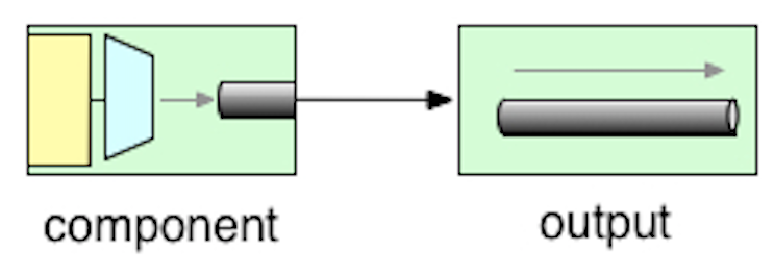
\epsfig{file=integration-module-output-channel.eps, height=.8in, width=2in}
\caption{Source Module Basic Components}
\label{fig:sourcembc}
\end{figure}
\subsection{Module Integrations: Sink}
The sink's responsibility is to convert message's in a stream to the format that can be 
consumed by the external agent and transmit the data to the agent. 
There are 2 types of sinks: Counter/Gauge and Delegate.  
A counter/gauge is a specialized sink increments a field on a datastore every time a 
message is received refer to the (Analytics Section) for more information.  A delegate 
sink's responsibility is to translate the XD message to the format that can be used by the
 external agent and dispatch that data to the agent or store the data in the specified 
 repository. \par  
 The basic sink is comprised of a "input" channel and a integration bean.
 The "input channel " will receive all messages from the stream and will and dispatch the
 messages to the integration bean. figure~\ref{fig:sinkmbc}. It is the responsibility of 
 the integration bean to implement retry behavior in cases of failure. In the current set 
 of XD sinks this behavior can be configured when the user constructs the stream by setting
 the parameters for the sink.  Each sink has different features so please review the 
 documentation on what features are available.\par
\begin{figure}
\centering
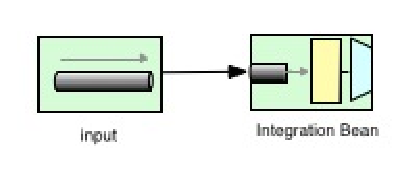
\epsfig{file=integration-module-input-channel.eps, height=.8in, width=2in}
\caption{Sink Module Basic Components}
\label{fig:sinkmbc}
\end{figure}
\subsection{Module Integrations: Job}
Spring XD uses Spring batch \cite{spring-batch-reference} as its foundation for implementing
job modules.  Jobs enables users to execute enterprise batch processes within the XD application. 
Jobs are typically used when running long lasting enterprise tasks that are transactionally 
sensitive.  Thus in cases that the job fails, a job can be designed to be restarted and 
pickup where it left off or rollback the changes that were in transaction.\par
A job is typical comprised of a job definition along with the supporting 
bean(s) as shown in figure~\ref{fig:batchmbc}.
In some cases the job definition alone is sufficient to implement the desired behavior.\par
\begin{figure}
\centering
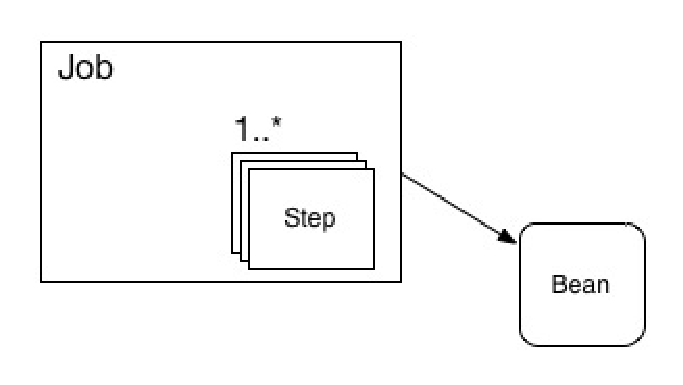
\epsfig{file=integration-batch.eps, height=.8in, width=2in}
\caption{Batch Basic Components}
\label{fig:batchmbc}
\end{figure}

\subsection{Deployment}
Integration Modules are deployed in the modules directory and are segregated in 
subdirectories by type: modules/source, modules/sink and modules/job.  
These modules are dynamically loaded when a stream or job is created that requires that 
specific module.  Once loaded, they are stored in Java's classloader and will not be 
reloaded (until the XD container is restarted).  Besides the pre-existing integration 
modules that come with the XD installation a user may create their own integration 
modules. \par

\subsection{Integration Examples}
With the advent of microservices \cite{microservices-pattern} applications are becoming 
evermore integrated.  In cases where an agent needs access to microservices but does not 
have the capability to transmit the request via the API presented, or an agent needs to 
take the results of a microservice and transmit it to  an external agent in the agent's 
accepted format, XD can bridge that chasm. 
An example of this would be if we needed a service that would receive sensor data via mqtt 
and write that the data to hdfs. The following stream would be used to do this: "mqtt|hdfs".
Another example of this would be a scenario if a database is being updated by a service 
but while the database is updated we need to update a mongo collection 
with this data.  This can be done by creating a stream that would monitor a table(s) 
retrieve changes and write the results to the mongo collection.  This would be 
represented by the following stream: 
"jdbc --fixedDelay=1 --split=1 --query='select * from testfoo where tag = 0' --update=
'update testfoo set tag=1 where fooid in (:fooid)'|log" 
\begin{description}
\item[Example Source] \hfill \\
jdbc - is a poller source that will execute a query against a database and generate a 
message for each row that is retrieved.  \cite{jdbc-module}
mqtt - is a event driven source that awaits for mqtt messages to be received once the message is
 received the payload of the message is sent as an XD message to the next module in the 
 stream.  \cite{mqtt-module}
\item[Example Sink] \hfill \\
Mongo - The Mongo sink writes messages into a Mongo collection \cite{mongo-module}
hdfs - writes messages to the specified location on a hadoop instance. \cite{hadoop-hdfs-module}
\item[Example Job] \hfill \\
filejdbc -A module which loads CSV files into a JDBC table\par
\end{description}
